\chapter{Data background}

In this chapter, let us briefly mention the most important parts of the biology of the brain and the physics behind the measuring techniques that are necessary to understand the rest of this thesis. In the beginning, it is important to emphasize that the brain is incredibly complex, and it is above the scope of this work to discuss its biological nature in detail. For further information, we highly recommend the book \textit{Neuroscience: exploring the brain} by Bear et al. \cite{bear_neuroscience_2016}

\section{The human brain}

First of all, by the term \enquote{the brain}, we refer to the cerebrum, the largest part responsible for, for example, conscious thoughts and actions. Figure \ref{fig:brain_cerebrum_illustration} shows its shape and location.

\begin{figure}
  \begin{center}
    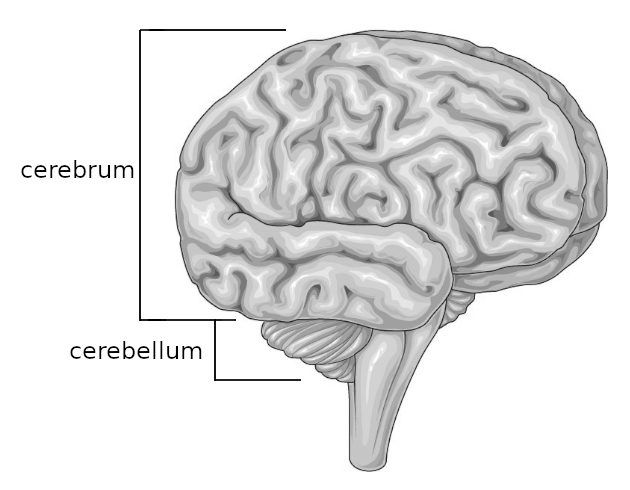
\includegraphics[width=6.3cm]{images/brain/brain_cerebrum_cerebellum_II.png}
  \end{center}
  % https://smart.servier.com/smart_image/smart-brain-overview/
  \caption[An artistic illustration showing cerebrum and cerebellum]{An artistic illustration showing cerebrum and cerebellum. Image adapted from Servier Medical Art, CC BY 4.0.}
  \label{fig:brain_cerebrum_illustration}
\end{figure}

The brain consists of various types of cells. Let us focus only on neurons, specialized cells that transmit information through electrical and chemical signals, because they are responsible for cognitive processes such as thinking and memory formation. The neuron structure is shown in Figure \ref{fig:neuron_illustration}. It consists of a cell body, dendrites and an axon. Cell body acts as neuron's central processing unit, while dendrites and axon enable neuron to receive and transmit electrochemical signals. 

In the brain, neurons are organized as shown in Figure \ref{fig:brain_matter_illustration}. The cell bodies form a layer called gray matter on the brain's surface (2.5 mm thick on average). Gray matter is crucial for processing and integrating information within the brain. The axons connecting the cell bodies fill the inner part of the brain and form a tissue called white matter. The primary function of white matter is to rapidly transmit signals between different areas of gray matter. The axons could be up to one meter long and form axonal bundles, where a few axons are organized in parallel. \cite{bear_neuroscience_2016}

\begin{figure}
  \begin{center}
    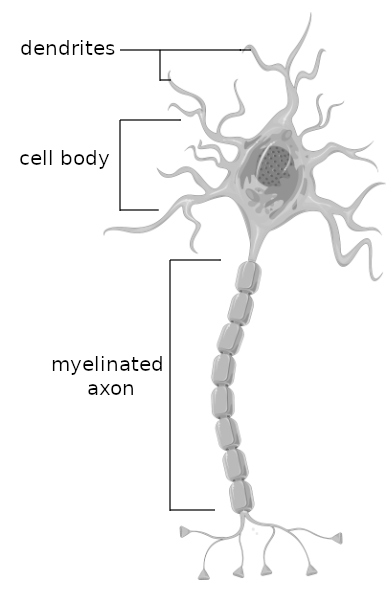
\includegraphics[width=5cm]{images/brain/neurone_II.png}
  \end{center}
  % https://smart.servier.com/smart_image/smart-neuron-overview/
  \caption[An artistic illustration of a neuron]{An artistic illustration of a neuron. The axon is myelinated (wrapped in fat); therefore, it is white, which gives name to the white matter. Image adapted from Servier Medical Art, CC BY 4.0.}
  %therefore, it is white. That is the reason, why is the white matter called white.
  \label{fig:neuron_illustration}
\end{figure}

\begin{figure}
  \begin{center}
    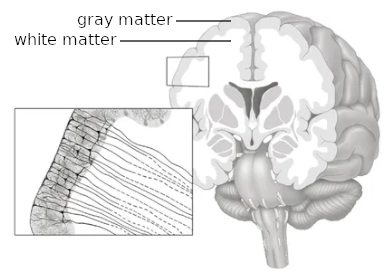
\includegraphics[width=6.3cm]{images/brain/brain_matter_illustration_II.png}
  \end{center}
  \caption[An artistic illustration of gray and white matter]{The brain comprises gray matter in the outer layer and white matter in the inner layer. The lines in the zoomed in diagram show axonal pathways leaving gray matter. An artistic illustration was created by Emma Vought, CC BY 4.0, and captions were added. \cite{bonilha_gray_2015}}
  \label{fig:brain_matter_illustration}
\end{figure}

\section{Magnetic Resonance Imaging}\label{sec:MRI}

Magnetic resonance imaging (MRI) is a widely employed technique that can be used to obtain a detailed picture of the brain. This section briefly introduces how MRI works. However, it is a simplification, and we recommend the book \textit{Magnetic Resonance Imaging: Theory and Practice} by Vlaardingerbroek and Boer for further information. \cite{vlaardingerbroek_magnetic_2003,bear_neuroscience_2016}

There is a great number of hydrogen atoms in the human body, both in water and fat. The protons in hydrogen nuclei have their own magnetic field because of the spin magnetic moment of the protons. When placed in a strong magnetic field in the MRI machine, some of the protons align themselves in parallel with the field. \cite{cizkova_comparing_2022}

When an electromagnetic pulse with the same frequency as the spinning protons (radiofrequency) is applied, the alignment is temporarily changed because the protons absorb the energy from the pulse and spin out of equilibrium. When the pulse is over, they return to their original alignment, emitting energy in the process. This energy is detected by a radio receiver. The MRI process consists of repeated cycles of the pulses.\cite{bear_neuroscience_2016,cizkova_comparing_2022}

In classical MRI, the fact that protons in different tissues and fluids change their magnetization differently causes different intensities of emitted energy and different brightness of the resulting image. Based on that, it is possible to distinguish different types of tissue. \cite{bear_neuroscience_2016,cizkova_comparing_2022}

\subsection{Diffusion weighted MRI}

What if we want to know not only that there is a white matter in a specific location but also the orientation of the axonal bundles connecting different areas of gray matter? This is when diffusion-weighted MRI (DW-MRI) is useful.

Diffusion is a process of transporting matter from one place to another by a random movement of molecules. The water in the brain (used in the MRI measurement as described above) also exhibits diffusion movement. Water diffuses much more easily along the axon membranes than across the axonal fibers. This fact is used to estimate the direction of axonal bundles by comparing the position of water molecules in subsequent MRI images. As a result, we obtain an estimation of axon fiber direction in each voxel in the resulting 3D image. \cite{bear_neuroscience_2016,jones_diffusion_2011,calamante_seven_2019}

For more details, we recommend a book \textit{Diffusion MRI: theory, methods, and applications} by D. K. Jones. \cite{jones_diffusion_2011}

\section{Electroencephalography}

In the previous section, we discussed MRI, which was used to measure the structural connectivity data in this thesis.\footnote{MRI could be used to measure function as well; so-called functional MRI is used, for example, for the reconstruction of resting state functional connectivity. However, we did not work with such data.} But how do we measure the function?

The communication and information processing in neurons is conducted via electrical signal transmission. The principle of electroencephalography (EEG) lies in measuring the difference in electrical potential caused by the brain activity between electrodes attached to the scalp. \cite{howseman_electroencephalographic_1999, st_louis_electroencephalography_2016, cooper_eeg_1974} We recommend a book \textit{EEG Technology} by Cooper, Osselton, and Shaw for more detailed information about EEG. \cite{cooper_eeg_1974}

The measurement has a temporal resolution in the range of milliseconds. Because of that, it is a suitable tool for recording the rapidly changing patterns of brain activity. However, it suffers from poor spatial resolution, which makes it difficult to infer the exact locations in the brain where the neural activity comes from. It is caused by the fact that the signal is a sum of activity generated by large groups of neurons under the electrodes weighted by the distance to the electrodes and the estimation of the signal sources is hard. \cite{howseman_electroencephalographic_1999, st_louis_electroencephalography_2016,michel_eeg_2019}

The EEG measurement results in one time series per electrode placed on the skull. However, what we truly want to know is the activation time series of specific locations inside the brain. We could perform source reconstruction to estimate the current sources that best fit the data to obtain activation time series per ROI instead of per electrode. See Figure \ref{fig:EEG} for illustration. The estimation process is complicated because the brain surface gray matter is folded, and the current spreads differently in different tissues in the brain. For an exact mathematical formulation of the source reconstruction problem and an overview of methods for solving the inverse problem, see \textit{Review on solving the inverse problem in EEG source analysis} by Grech et al. \cite{grech_review_2008}

\begin{figure}
  \begin{center}
    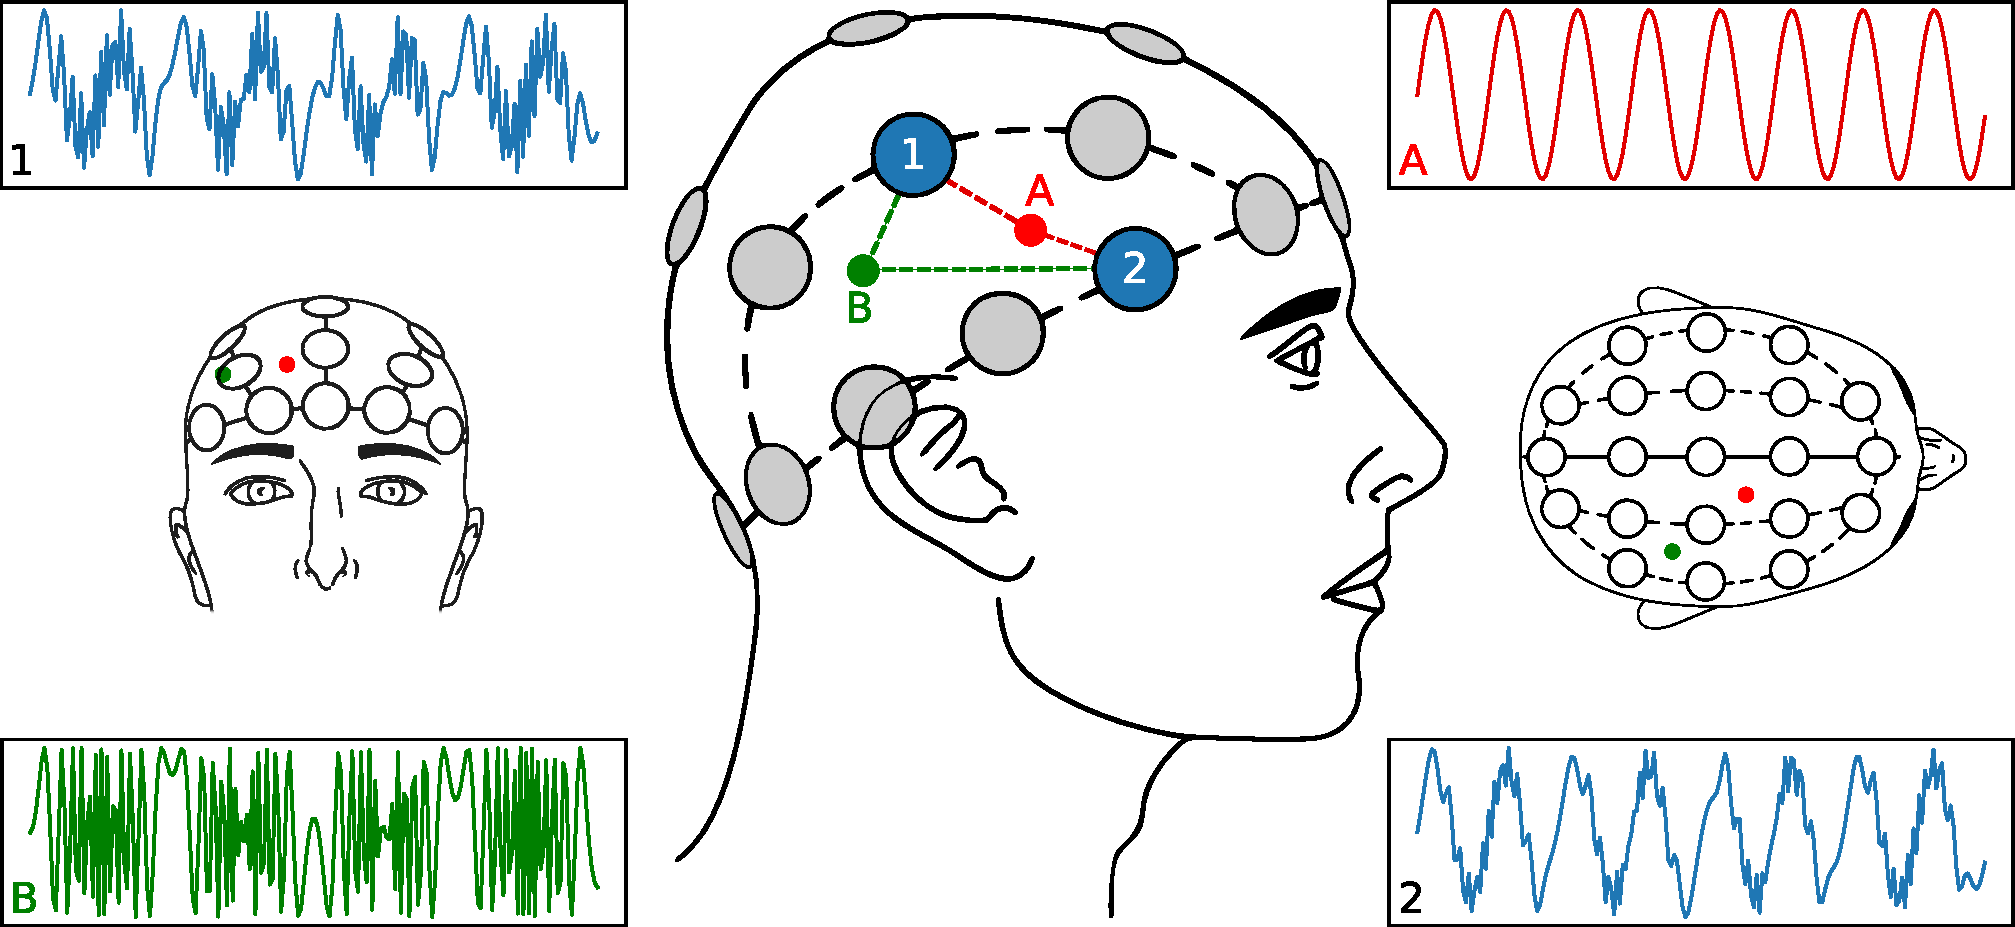
\includegraphics[width=\textwidth]{images/brain/EEG_source_reconstruction.png.pdf}
  \end{center}
  \caption[An artistic illustration of EEG and its source reconstruction]{An illustration of EEG and its source reconstruction. Let us consider measurement sites 1 and 2 and their corresponding time series. The source reconstruction process aims to determine the activity at some places inside the skull, for example, A and B. Head and EEG montage images adapted from Servier Medical Art, CC BY 4.0.}
  \label{fig:EEG}
\end{figure}

\subsection{iEEG}

Intracranial electroencephalography (iEEG) is an invasive measuring method; the electrodes are implanted into the skull. Because of that, the source reconstruction is not necessary. It has much better spatial resolution than the scalp EEG described above and also a high signal-to-noise ratio because it measures the neuronal responses around its origin. On top of that, it enables direct electrical stimulation of the brain by applying precise electric pulses to specific brain areas.
All of this makes iEEG one of the best methods to measure the dynamic changes of brain activity across time and space after a stimulation. However, due to ethical issues with implanting electrodes in the human brain, iEEG recordings are typically performed in drug-resistant epilepsy patients for clinical purposes, which makes iEEG less common than other noninvasive neuroimaging methods. In this thesis, we use data from the \textit{The Functional Brain Tractography project} (F-TRACT), which was also performed in epileptic patients. \cite{axmacher_what_2023,seguin_communication_2023}

\subsection{TMS-EEG}

Transcranial magnetic stimulation EEG (TMS-EEG) is a noninvasive alternative to iEEG when we want to study the reaction of the brain to a stimulation. It combines scalp EEG measurement with TMS stimulation when applying magnetic pulses over the scalp triggers electrical activity in specific brain regions. The stimulation is produced by a brief electric current passing through a magnetic coil, which generates a brief magnetic field of high intensity. The magnetic field induces an electric field in the brain, and the voltage and induced currents excite the neurons in the area. \cite{hallett_transcranial_2007}



